\documentclass[11pt]{article}
\usepackage{caption}
\usepackage{anysize}
\usepackage{fancyhdr}
\usepackage{graphicx}
\usepackage{subcaption}
\usepackage{color}
\usepackage{balance}
\usepackage{lipsum}
\usepackage{multirow}
\usepackage{multicol}
\usepackage{booktabs}

% REQUIRED PACKAGES FOR TIKZ DRAWINGS %
\usepackage{tikz}
\usetikzlibrary{positioning}
\usetikzlibrary{spy}
\usetikzlibrary{decorations.fractals}

\title{}
\date{}
\begin{document}
\maketitle

%% %%%%%%%%%  %%
%% Furnace and Tube %%
%% %%%%%%%%%  %%

\section*{Furnace and Tube}

\begin{center}
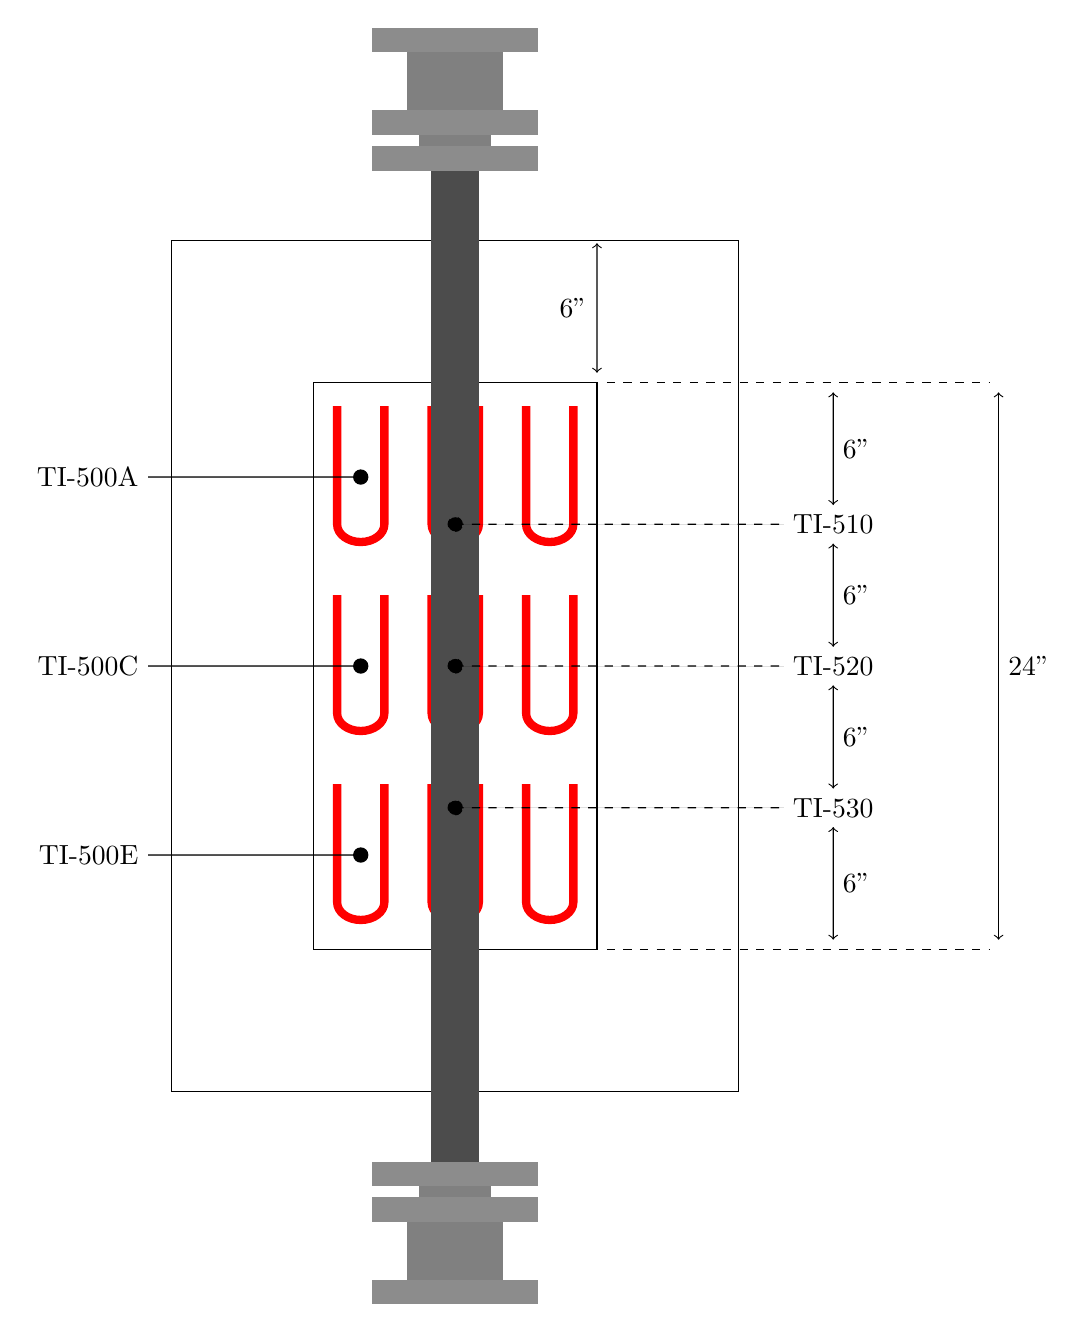
\begin{tikzpicture}[scale=0.3]
	\node (toprighthot) at (6,12) {};
	\node (bottomlefthot) at (-6,-12) {};
	\node (bottomrighthot) at (6,-12) {};
	\node (toplefthot) at (-6,12) {};
	\node (toprightbox) at (12,18) {};
	\node (topleftbox) at (-12,18) {};
	\node (bottomleftbox) at (-12,18) {};
	\node (bottomrightbox) at (12,-18) {};
	% Furnace Box %
	\draw (-12,-18) rectangle  (12,18);
	% Hot Zone %
	\filldraw [fill=red, fill opacity=0] (bottomlefthot) rectangle (toprighthot);
	% Elements %
	\foreach \y in {11, 3, -5}
		\foreach \x in {-5, -1, 3}
			{\draw [red,line width=3] (\x,\y) -- ++(0,-5) arc (180:360:1 and 0.75) -- ++(0,5);}
	% Tube %
	\filldraw [black!70!white] (-1,-27) rectangle (1,27);
	% Top Bucket %
	\filldraw [gray] (-1.5,21) rectangle (1.5,23.5);
	\filldraw [gray] (-2,23.5) rectangle (2,27);
	\filldraw [gray!90!white] (-3.5,21) rectangle (3.5,22);
	\filldraw [gray!90!white] (-3.5,22.5) rectangle (3.5,23.5);
	\filldraw [gray!90!white] (-3.5,26) rectangle (3.5,27);
	% Bottom Bucket %
	\filldraw [gray] (-1.5,-21) rectangle (1.5,-23.5);
	\filldraw [gray] (-2,-23.5) rectangle (2,-27);
	\filldraw [gray!90!white] (-3.5,-21) rectangle (3.5,-22);
	\filldraw [gray!90!white] (-3.5,-22.5) rectangle (3.5,-23.5);
	\filldraw [gray!90!white] (-3.5,-26) rectangle (3.5,-27);
	% Skin Thermocouples %
	\filldraw [black] (0,6) circle (0.3) [dashed] -- (16,6) node (ti510) [fill=white] {TI-510};
	\filldraw [black] (0,0) circle (0.3) [dashed] -- (16,0) node (ti520) [fill=white] {TI-520};
	\filldraw [black] (0,-6) circle (0.3) [dashed] -- (16,-6) node (ti530) [fill=white] {TI-530};
	\node (top510) at (16,12) {};
	\node (topright510) at (23,12) {};
	\node (bottom530) at (16,-12) {};
	\node (bottomright530) at (23,-12) {};
	\draw [<->] (top510) to node [auto] {6"} (ti510);
	\draw [<->] (ti510) to node [auto] {6"} (ti520);
	\draw [<->] (ti520) to node [auto] {6"} (ti530);
	\draw [<->] (ti530) to node [auto] {6"} (bottom530);
	\draw [<->] (topright510) to node [auto] {24"} (bottomright530);
	\draw [dashed] (toprighthot) -- (topright510);
	\draw [dashed] (bottomrighthot) -- (bottomright530);
	\draw [<->] (toprighthot) to node [auto] {6"} ++(0,5.9);
	% Element Thermocouples %
	\filldraw [black] (-4,8) circle (0.3) -- (-13,8) node (ti510) [anchor=east] {TI-500A};
	\filldraw [black] (-4,0) circle (0.3) -- (-13,0) node (ti520) [anchor=east] {TI-500C};
	\filldraw [black] (-4,-8) circle (0.3) -- (-13,-8) node (ti530) [anchor=east] {TI-500E};

\end{tikzpicture}
\end{center}

%% %%% %%
%% Lance %%
%% %%% %%	
	
\begin{center}
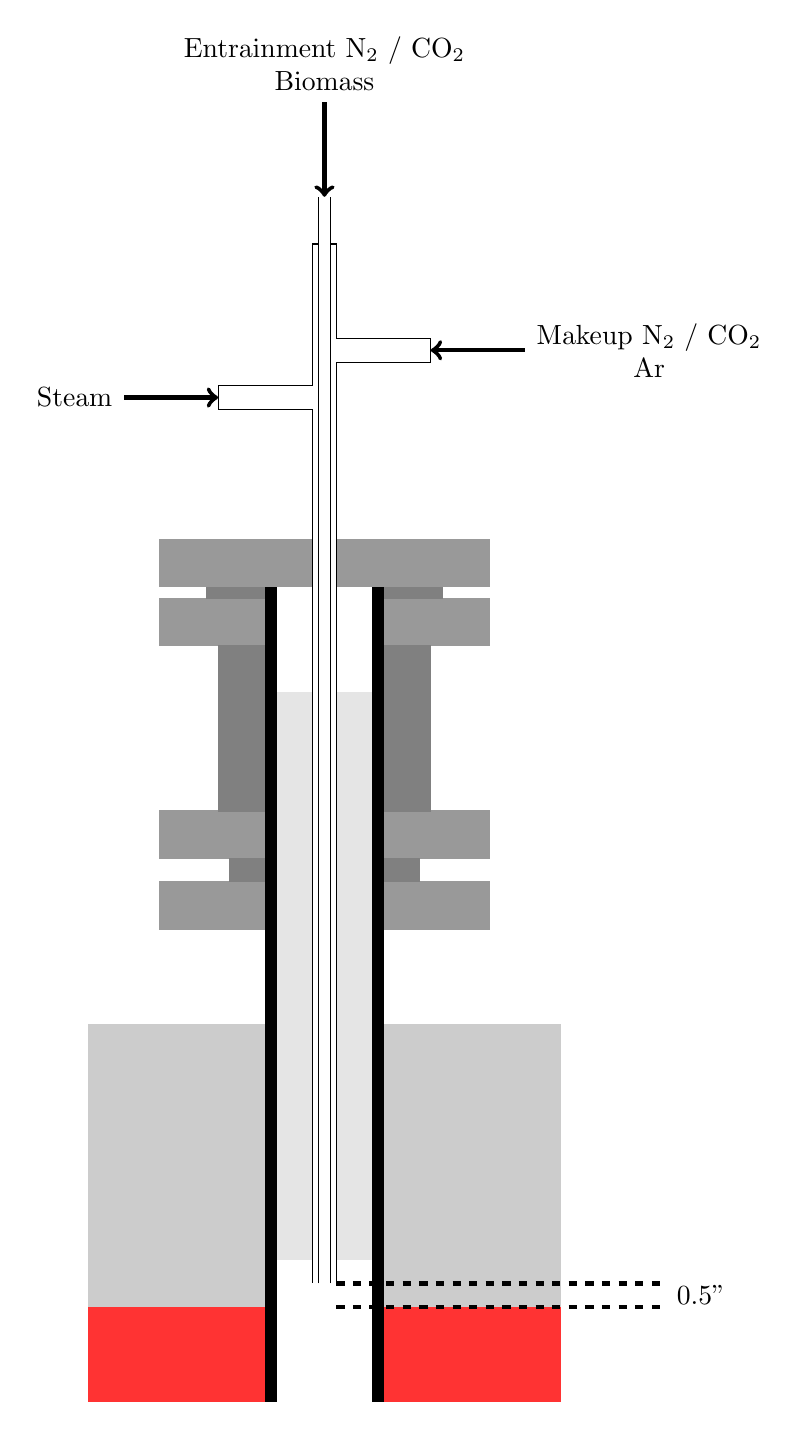
\begin{tikzpicture}[scale=.6]
	% Bucket Seal %
	\filldraw [gray!80] (-3.5,14) rectangle (3.5,15);
	\filldraw [gray!80] (-3.5,8) rectangle (3.5,9);
	\filldraw [gray!80] (-3.5,9.5) rectangle (3.5,10.5);
	\filldraw [gray] (-2.25,10.5) rectangle (2.25,14);
	\filldraw [gray] (-2,9) rectangle (2,9.5);
	\filldraw [gray] (-2.5,15)  rectangle (2.5,15.25);
	\filldraw [gray!80] (-3.5,15.25) rectangle (3.5,16.25);
	% Furnace and Tube %
	\fill [color=gray!40] (-5,0) rectangle (5,6);
	\fill [color=red!80] (-5,0) rectangle (5,-2);
	\fill [color=white] (-1,-2) rectangle (1,15.25);
	% Lance Insulation %
	\filldraw [gray!20] (-1,1) rectangle (1,13);
	\fill [color=black] (-1.25,-2) rectangle (-1,15.25);
	\fill [color=black] (1.25,-2) rectangle (1,15.25);
	
	% Annular Tube %
	\draw [fill=white] (.25,0.5) -- ++ (0,14.5) -- ++ (0,5) -- ++ (2,0) -- ++ (0,.25) node (backup){} -- ++ (0,.25) -- ++ (-2,0) -- ++ (0,2) -- ++ (-.5,0) -- ++ (0,-3) -- ++ (-2,0) -- ++ (0,-.25) node (steam){} -- ++ (0,-.25) -- ++ (2,0) -- ++ (0,-4) -- ++ (0,-14.5);
	% Center Tube %
	\fill [color=white] (-1/8,0.5) rectangle (1/8,23);
	\draw (-1/8,0.5) -- ++ (0,23);
	\draw (1/8,0.5) -- ++ (0,23);
	% Labels %
	\draw [<-,ultra thick] (steam.center) -- ++ (-2,0) node [anchor=east] {Steam};
	\draw [<-,ultra thick] (backup.center) -- ++ (2,0) node [anchor=west, align=center] {Makeup N$_2$ / CO$_2$ \\ Ar};
	\draw [<-,ultra thick] (0,23.5) -- ++ (0,2) node [align=center, anchor=south] {Entrainment  N$_2$ / CO$_2$ \\ Biomass};
	\draw [dashed, ultra thick] (.25,.5) -- ++ (7,0);
	\draw [dashed, ultra thick] (0.25,0) -- ++ (7,0);
	\draw (7.25,0.25) node [anchor=west] {0.5"};
	
\end{tikzpicture}
\end{center}


%% %%%%%%%  %%
%% Flow Diagram %%
%% %%%%%%%  %%

%\begin{center}
%\begin{tikzpicture}[scale=1,
%	box/.style={rectangle,draw,align=center}
%	]
%	\node [box] (gasifier)	{Gasifier};
%	\node (lance)			[above=of gasifier]	{};
%	\node [box] (ako)		[below=of gasifier]	{Ash \\ Knockout};
%	\node [box] (filters)		[right=of ako]		{Candle \\Filters};
%	\node [box] (vls)		[right=of filters]	{VLS};
%	\node [box] (fabfilters)	[below=of vls]		{Cloth \\ Filters};
%	\node (tee)			[below=of fabfilters]	{};
%	\node [box] (pcv)		[below=of tee]		{PCV};
%	\node [box,rounded corners] (feeder)		[left=of lance]	{Biomass \\Feeder};
%	\node [box] (analytical)	[left=of tee]		{Analytical};
%	\node (vent)			[below=of pcv]		{Vent};
%	
%	\node [box] (gas)		[above left=of lance]	{Gas \\ Supply};
%	\node [box] (steam)		[above right=of lance]	{Steam \\ Generator};
%	
%	\draw [->] (feeder) [ultra thick] 				to (gasifier);
%	\draw [->] (gasifier) [ultra thick] 			to (ako);
%	\draw [->] (ako) [ultra thick] 				to (filters);
%	\draw [->] (filters) [ultra thick] 				to (vls);
%	\draw [->] (vls) [ultra thick] 				to (fabfilters);
%	\draw [->] (fabfilters) [ultra thick] 			to (pcv);
%	\draw [->] (tee.center) [ultra thick] 	to (analytical);
%	\draw [->] (pcv) [ultra thick]				to (vent) ;
%
%\end{tikzpicture}
%\end{center}


%% %%%%%%%%  %%
%% Biomass Feeder %%
%% %%%%%%%%  %%

\section*{Biomass Feeder}

\begin{center}
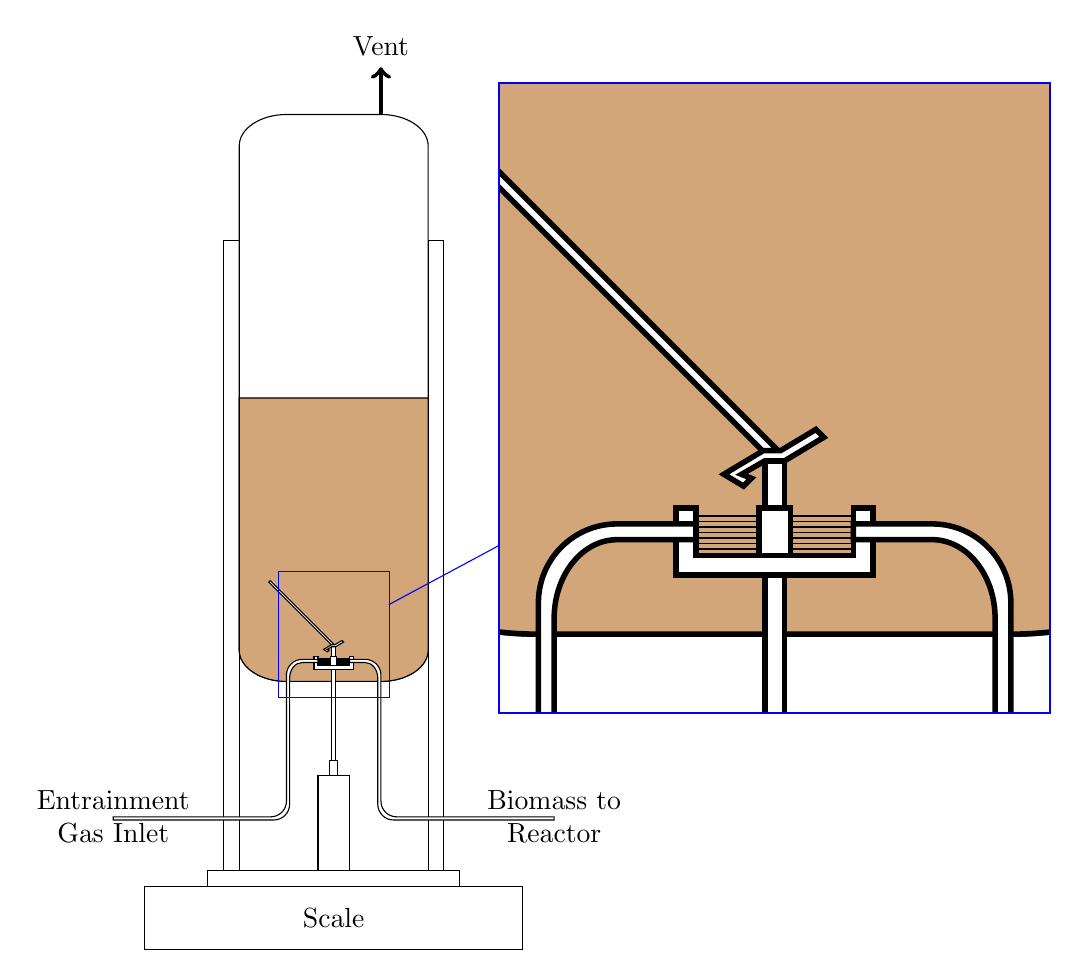
\begin{tikzpicture}[scale=0.2,
	spy using outlines={rectangle, magnification=5, width=7cm, height=8cm, connect spies}]

	% Vessel %
	\draw (-6,-	16) -- (-6,16) arc (180:90:3 and 2) -- (3,18) arc (90:0:3 and 2) -- (6,16) -- (6,-16) arc (0:-90:3 and 2) -- (-3,-18) arc  (-90:-180:3 and 2);
	\draw [fill=brown!70!white] (-6,-16) -- (-6,0) -- (6,0) -- (6,-16) arc (0:-90:3 and 2) -- (-3,-18) arc  (-90:-180:3 and 2);
	% Base %
	\draw (-7,-30) rectangle (-6,10);
	\draw (6,-30) rectangle (7,10);
	\draw (-8,-31) rectangle (8,-30);
	% Scale %
	\draw (-12,-35) rectangle (12,-31) node [pos=.5]{Scale};
	% Shaft %
	\draw [fill=white] (-.25/2,-24) rectangle (0.25/2,-17.25);
	% Motor %
	\draw (-1,-30) rectangle (1,-24);
	\draw [fill=white] (-0.25,-24) rectangle (0.25,-23);
	% Brush %
	\foreach \y in {-16.5, -16.57, ..., -17} \draw (-1,\y) [ultra thin] -- (1,\y);
	\draw [fill=white] (-.2,-17) rectangle (.2,-16.4);
	\draw [fill=white] (-.125,-16.4) rectangle (.125,-15.8);
	% Wipers %
	\draw [fill=white] (-.125,-15.7) -- ++ (-4,4) -- ++ (0.1,0.1) -- ++ (4.1,-4.1) --cycle;
	\draw [fill=white] (-.125,-15.8) -- (.125,-15.8) -- ++ (0.5,0.3) -- ++ (-0.1,0.1) -- ++ (-0.45,-0.27) -- ++ (-0.22,0) -- ++ (-0.5,-0.3) -- ++ (0.25,-0.15) -- ++ (0.1,0.1) -- ++ (-0.125,0.05) -- cycle;
	% Cup %
	\draw [fill=white] (-1,-17) -- ++(2,0) -- ++(0,.6) -- ++(0.25,0) -- ++(0,-.4) -- ++(0,-.45) -- ++(-2.5,0) -- ++(0,0.45) -- ++(0,0.4) -- ++(0.25,0) -- cycle;
	% Flex Lines %
	\draw [fill=white] (-1,-16.6) -- ++(-1,0) arc (90:180:1) -- ++(0,-8) arc (0:-90:1) -- ++ (-10,0)  node [align=center] {Entrainment \\ Gas Inlet} -- ++(0,-.2) -- ++(10.2,0) arc(-90:0:1) -- ++ (0,8) arc (180:90:.8 and 1) -- ++(1,0) --cycle ;
	\draw [fill=white] (1,-16.6) -- ++(1,0) arc (90:0:1) -- ++(0,-8) arc (180:270:1) -- ++ (10,0) node [align=center] {Biomass to \\ Reactor} -- ++(0,-.2) -- ++(-10.2,0) arc(-90:-180:1) -- ++ (0,8) arc (0:90:.8 and 1) -- ++(-1,0) --cycle ;
	\draw [->] (3,18) [ultra thick] -- (3,21) node [anchor=south] {Vent};
	% Spy Glass %
	\spy [blue] on (0,-3)
	in node at (28,0);
\end{tikzpicture}
\end{center}

%% %%%%%%%%%%  %%
%%  Steam Generator    %%
%% %%%%%%%%%%  %%

\section*{Steam Generator}

\begin{center}
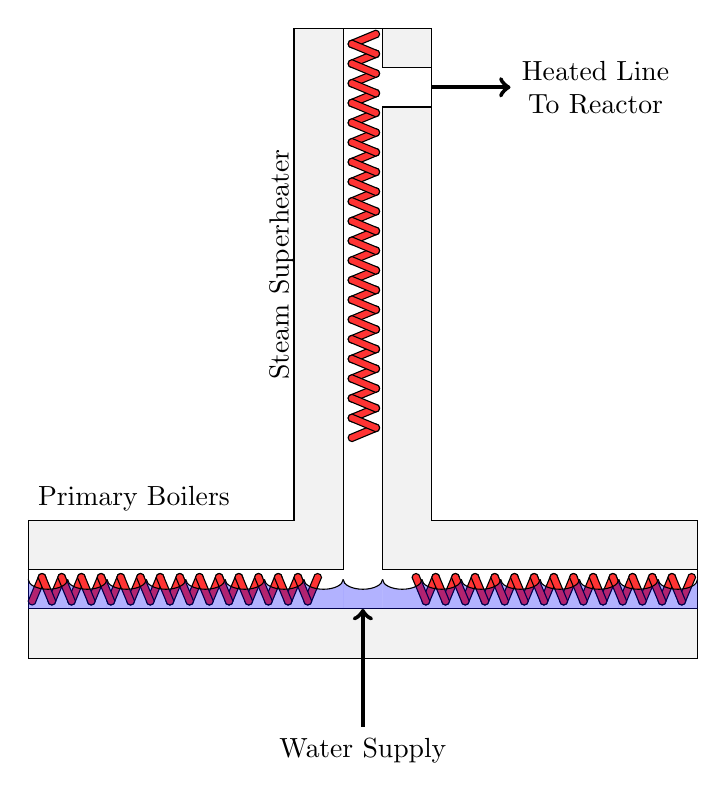
\begin{tikzpicture}[scale=0.5]
	\draw [fill=gray!10] (0,0) -- ++ (17,0) -- ++ (0,3.5) -- ++ (-6.75,0) -- ++ (0,12.5) -- ++ (-3.5,0) -- ++ (0,-12.5) -- ++ (-6.75,0) -- ++ (0,-3.5);
	\draw [fill=white] (0,1.25) -- ++ (17,0) -- ++ (0,1) -- ++ (-8,0) -- ++ (0,11.75) -- ++ (1.25,0) -- ++ (0,1) -- ++ (-1.25,0) -- ++ (0,1) -- ++ (-1,0) -- ++ (0,-13.75) -- ++ (-8,0) -- ++ (0,-1);
	% Top Element %
	\foreach \y in {5.5, 6, ..., 15.5} \draw [fill=red!80] (8.225,\y) arc (-90:-270:0.1) --  ++ (.6,.25) arc (90:-90:0.1) --cycle;
	\foreach \y in {5.75, 6.25, ..., 15.5} \draw [fill=red!80] (8.825,\y) arc (-90:90:0.1) --  ++ (-.6,.25) arc (90:270:0.1) --cycle;
	% Left Element %
	\foreach \x in {0, .5, ..., 7} \draw [fill=red!80] (\x,1.45) arc (-180:0:0.1) --  ++ (.25,.6) arc (0:180:0.1) --cycle;
	\foreach \x in {.25, .75, ..., 7} \draw [fill=red!80] (\x,2.05) arc (180:0:0.1) --  ++ (.25,-.6) arc (0:-180:0.1) --cycle;
	% Right Element %
	\foreach \x in {10, 10.5, ..., 16.75} \draw [fill=red!80] (\x,1.45) arc (-180:0:0.1) --  ++ (.25,.6) arc (0:180:0.1) --cycle;
	\foreach \x in {9.75, 10.25, ..., 16.5} \draw [fill=red!80] (\x,2.05) arc (180:0:0.1) --  ++ (.25,-.6) arc (0:-180:0.1) --cycle;
	% Water %
	\foreach \x in {0,1,...,16} \fill [fill=blue,fill opacity=0.3] (\x,2)  arc (180:360:.5 and .25) -- ++ (0,-.75) -- ++ (-1,0) -- ++ (0,.75);
	\foreach \x in {0,1,...,16} \draw  (\x,2)  arc (180:360:.5 and .25);
	% Lines and Text %
	\draw [<-,ultra thick] (8.5,1.25) -- ++ (0,-3) node [anchor=north]{Water Supply};
	\draw [->,ultra thick] (10.25,14.5) -- ++ (2,0) node [anchor=west, align=center]{Heated Line \\ To Reactor};
	\draw (0,3.5) node [anchor=south west,align=center] {Primary Boilers};
	\draw (7,10) node [anchor=south,align=center,rotate=90] {Steam Superheater};
\end{tikzpicture}
\end{center}

%% %%%%%%%%  %%
%%  Ash Knockout   %%
%% %%%%%%%%  %%

\section*{Ash Knockout}

\begin{center}
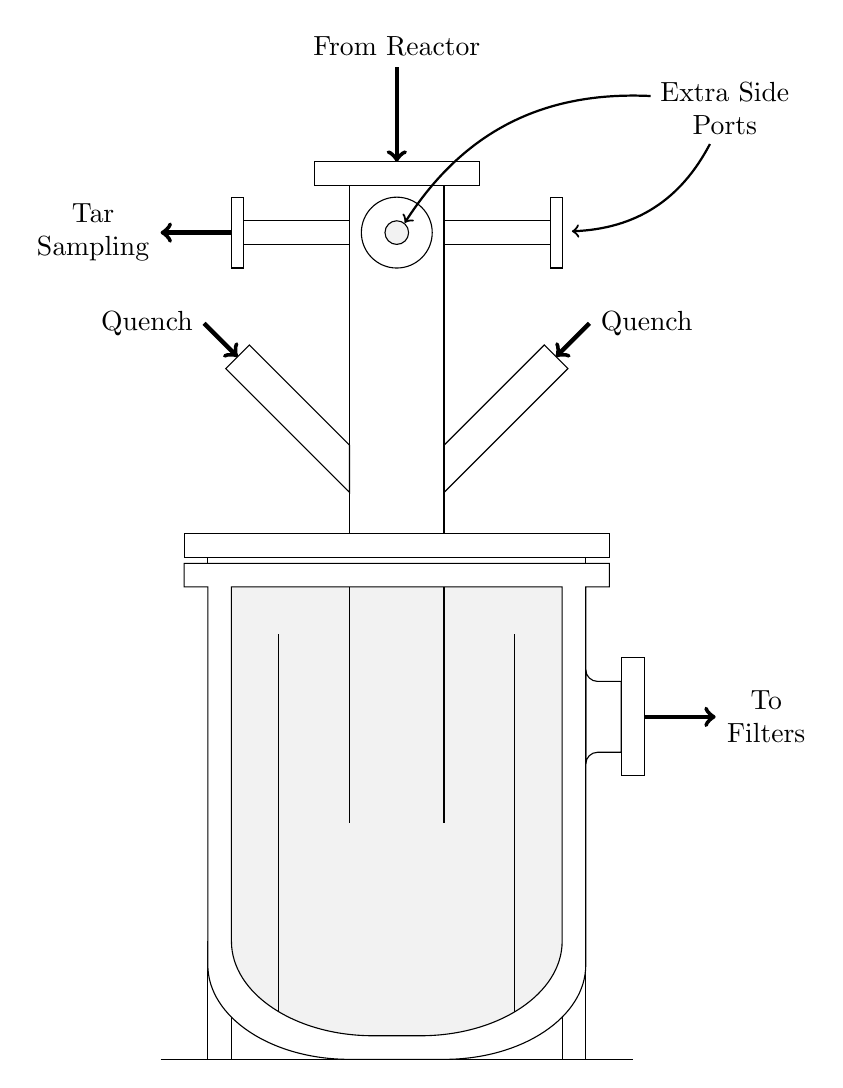
\begin{tikzpicture}[scale=0.3]

	% Feet %
	\draw (-8,0) rectangle (-7,5);
	\draw (8,0) rectangle (7,5);
	\draw (-10,0) -- (10,0);
	% Vessel %
	\draw [fill=white](-9,21) -- (9,21) -- (9,20) -- (8,20) -- (8,4) arc (0:-90:6 and 4) -- (-2,0) arc (-90:-180:6 and 4) -- (-8,20) -- (-9,20) -- cycle;
	\draw [fill=gray!10!white] (-7,20) -- (7,20) -- (7,5) arc (0:-90:6 and 4) -- (-1,1) arc (-90:-180:6 and 4) -- cycle;
	% Baffles %
	\draw (-2,20) -- (-2,10);
	\draw (2,20) -- (2,10);
	\draw (-5,18) -- (-5,2);
	\draw (5,18) -- (5,2);
	% Gasket %
	\draw (-8,21) rectangle (8,21.25);
	% Lid %
	\draw (-9,21.25) rectangle (9,22.25);
	% Chimney %
	\draw (-2,22.25) rectangle (2,37);
	% Flange %
	\draw (-3.5,37) rectangle (3.5,38);
	\draw [<-] (0,38) [ultra thick] to (0,42) node [anchor=south] {From Reactor};
	% Quench %
	\draw (-2,24) -- (-2,26) -- ++ (135:6)  -- ++ (-0.5,-0.5) node (quench1) {} -- ++ (-0.5,-0.5) --cycle;
	\draw (2,24) -- (2,26) -- ++ (45:6) -- ++ (0.5,-0.5)  node (quench2) {} -- ++ (0.5,-0.5) --cycle;
	\draw [<-, ultra thick] (quench1.center) to ++(135:2) node [align=center, anchor = east] {Quench};
	\draw [<-, ultra thick] (quench2.center) to ++(45:2) node [align=center, anchor = west] {Quench};
	% Side Ports %
	\draw (-2,35.5) rectangle (-6.5,34.5);
	\draw (2,35.5) rectangle (6.5,34.5);
	\draw (-6.5,36.5) rectangle (-7,33.5);
	\draw (6.5,36.5) rectangle (7,33.5);
	\draw [->, ultra thick] (-7,35) -- ++ (-3,0) node [anchor=east,align=center] {Tar \\Sampling};
	\draw (0,35) circle (1.5);
	\draw [fill=gray!10] (0,35) circle (.5);
	\node (port1) at (0,35) {};
	\node (port2) at (7,35) {};
	\node (portlabel) [above right=of port2, align=center] {Extra Side \\ Ports};
	\draw [->, thick, bend right] (portlabel) to (port1);
	\draw [->, thick, bend left] (portlabel) to (port2);
	% Outlet %
	\draw (8,12.5) arc (-180:-270:.5) -- ++ (1,0) -- ++ (0,3) -- ++ (-1,0) arc (-90:-180:.5) --cycle;
	\draw (9.5,12) rectangle (10.5,17);
	\draw [->,ultra thick] (10.5,14.5) -- ++ (3,0) node [anchor=west,align=center] {To \\ Filters};
\end{tikzpicture}
\end{center}


%% %%%%%%  %%
%%  Ash Filters   %%
%% %%%%%%  %%

\section*{Ash Filters}

\begin{center}
\begin{tikzpicture}[scale=0.3]

	\draw (-3,0) rectangle (3,34);
	\draw (-4,0) rectangle (4,-1);
	\draw (-3,-1) rectangle (3,-1.25);
	\draw (-4,-1.25) rectangle (4,-2.25);
	\draw (-4,34) rectangle (4,35);
	\draw (-3,35) rectangle (3,35.25);
	\draw (-4,35.25) rectangle (4,36.25);
	\draw (0,6) circle (1);
	\draw (0,6) circle (2.5);
	\draw [<-, ultra thick] (0,6) -- ++(-5,4) node [anchor=east, align=center] {From Ash \\ Knockout};

	\draw (8,6) rectangle (14,40);
	\draw (7,6) rectangle (15,5);
	\draw (8,5) rectangle (14,4.75);
	\draw (7,4.75) rectangle (15,3.75);
	\draw (7,40) rectangle (15,41);
	\draw (8,41) rectangle (14,41.25);
	\draw (7,41.25) rectangle (15,42.25);

	\draw [fill=white] (-1.5,36.25) -- (-1.5,38.5) --++ (8,0) arc (90:0:0.5) --++ (0,-10) arc (180:360:1.875) --++ (0,4) arc (180:0:0.25) -- ++ (0,-4.25) arc (0:-180:2.375 and 2.125) --++ (0,10) arc (0:90:.25) -- (1.5, 38) -- (1.5,36.25);
	\draw (0.25,36.25) rectangle (1,38);
	\draw (-0.25,36.25) -- (-0.25,38) -- ++ (-.75,0)  -- (-1,36.25);
	\draw [->,ultra thick] (11,42.25) -- ++ (0,3) node [anchor=south,align=center] {To VLS};
\end{tikzpicture}
\end{center}


%% %%% %%
%%   VLS  %%
%% %%% %%

\section*{Vapor Liquid Separation}

\begin{center}
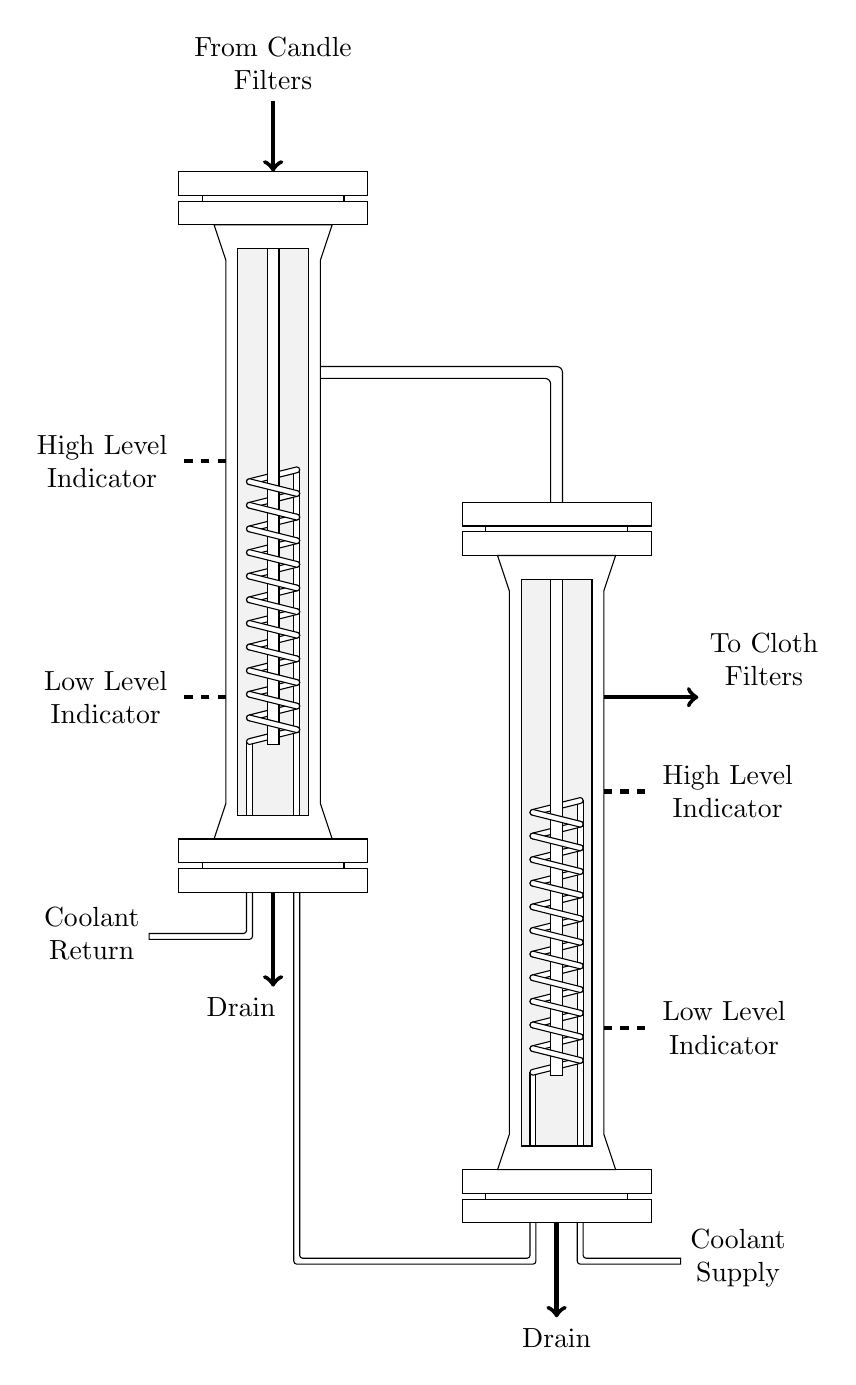
\begin{tikzpicture}[scale=0.3]

	%% First Vessel %%
	\draw (-2.5,0) -- (-2,1.5) --(-2,24.5) -- (-2.5,26) -- (2.5,26) -- (2,24.5) -- (2,1.5) -- (2.5,0) -- cycle;
	\draw (-4,0) rectangle (4,-1);
	\draw (-3,-1) rectangle (3,-1.25);
	\draw (-4,-1.25) rectangle (4,-2.25);
	\draw (-4,26) rectangle (4,27);
	\draw (-3,27) rectangle (3,27.25);
	\draw (-4,27.25) rectangle (4,28.25);
	\draw [fill=gray!10] (-1.5,1) rectangle (1.5,25);
	\draw [->,ultra thick] (0,-2.25) -- ++ (0,-4) node [anchor=north east,align=center,xshift=5] {Drain};
	\draw [<-,ultra thick] (0,28.25) -- ++ (0,3) node [anchor=south,align=center] {From Candle \\ Filters};
	%% First Vessel Loops %%
	\draw [fill=white] (1.125,15.625) rectangle (.875,1);
	\draw [fill=white] (-1.125,4.125) rectangle (-.875,1);
	\foreach \y in {4, 5, ..., 15} \draw [fill=white] (-1,\y) arc (-90:-270:0.125) --  ++ (2,.5) arc (90:-90:0.125) --cycle;
	\draw [fill=white] (-.25,25) rectangle (.25,4);
	\foreach \y in {4.5, 5.5, ..., 14.5} \draw [fill=white] (1,\y) arc (-90:90:0.125) --  ++ (-2,.5) arc (90:270:0.125) --cycle;
	\draw (-1.125,-2.25) -- ++ (0,-1.625) arc (0:-90:0.125) -- ++ (-4,0) node [anchor=east,align=center] {Coolant \\ Return}-- ++ (0,-0.25) -- ++ (4.25,0) arc (-90:0:0.125) -- ++ (0,1.875) ;
	%% Second Vessel %%
	\draw (9.5,-14) -- (10,-12.5) --(10,10.5) -- (9.5,12) -- (14.5,12) -- (14,10.5) -- (14,-12.5) -- (14.5,-14) -- cycle;
	\draw (8,-14) rectangle (16,-15);
	\draw (9,-15) rectangle (15,-15.25);
	\draw (8,-15.25) rectangle (16,-16.25);
	\draw (8,12) rectangle (16,13);
	\draw (9,13) rectangle (15,13.25);
	\draw (8,13.25) rectangle (16,14.25);
	\draw [fill=gray!10] (10.5,-13) rectangle (13.5,11);
	\draw [->,ultra thick] (14,6) -- ++ (4,0) node [anchor=south west,align=center] {To Cloth\\Filters};
	\draw [->,ultra thick]  (12,-16.25) -- ++ (0,-4) node [anchor=north,align=center] {Drain};
	%% Second Vessel Loops %%
	\draw [fill=white] (13.125,1.625) rectangle (12.875,-13);
	\draw [fill=white] (10.875,-9.875) rectangle (11.125,-13);
	\foreach \y in {-10, -9, ..., 1} \draw [fill=white] (11,\y) arc (-90:-270:0.125) --  ++ (2,.5) arc (90:-90:0.125) --cycle;
	\draw [fill=white] (11.75,11) rectangle (12.25,-10);
	\foreach \y in {-9.5, -8.5, ..., 0.5} \draw [fill=white] (13,\y) arc (-90:90:0.125) --  ++ (-2,.5) arc (90:270:0.125) --cycle;
	\draw (13.125,-16.25) -- ++ (0,-1.375) arc (180:270:0.125) -- ++ (4,0) node [anchor=west,align=center] {Coolant \\ Supply}-- ++ (0,-0.25) -- ++ (-4.25,0) arc (-90:-180:0.125) -- ++ (0,1.625) ;
	%% Lines Between %%
	\draw (2,20) -- ++ (10,0) arc (90:0:0.25) -- ++(0,-5.5)  ++ (-.5,0) -- ++ (0,5) arc (0:90:0.25) -- (2,19.5);
	\draw (0.875,-2.25) -- (0.875,-17.875) arc (180:270:0.125) -- (11,-18) arc (270:360:0.125) -- ++ (0,1.625) ++ (-0.25,0) -- ++ (0,-1.375) arc (0:-90:0.125) -- (1.25,-17.75) arc (-90:-180:0.125) -- ++ (0,15.375);
	%% Level Indicators %% 
	\draw [dashed,ultra thick] (-2,16) -- ++ (-2,0) node [anchor=east,align=center] {High Level \\Indicator};
	\draw [dashed,ultra thick] (-2,6) -- ++ (-2,0) node [anchor=east,align=center] {Low Level \\Indicator};
	\draw [dashed,ultra thick] (14,2) -- ++ (2,0) node [anchor=west,align=center] {High Level \\Indicator};
	\draw [dashed,ultra thick] (14,-8) -- ++ (2,0) node [anchor=west,align=center] {Low Level \\Indicator};
	
					
\end{tikzpicture}
\end{center}

\end{document}

